\documentclass{article}

\usepackage[margin=1in]{geometry}
\usepackage{amsmath}
\usepackage{graphicx}
\usepackage{booktabs}
\usepackage{multirow}
\usepackage{xcolor}

\title{Fused Attention for Scratchpad-Based Accelerators:\\Reducing Data Movement on the FlexASR Platform}

\author{
Varun Madan \and Rishabh Sharad Pomaje \\
Department of Computer Science, Department of Electrical Engineering \\
Stanford University\\
\texttt{\{rishabhp, vmadan\}@stanford.edu}
}

\begin{document}

\maketitle


%------------------------------------------------
% INTRODUCTION
%------------------------------------------------

\section*{Introduction}

The Transformer architecture~[2] has become the foundation of modern AI, powering large language models~[1] and multimodal systems. At its core is the \textit{scaled dot-product attention} mechanism:
\[
\text{Attention}(Q,K,V) =
\text{softmax}
\left(
\frac{QK^T}{\sqrt{d}}
\right)V
\]
where $N$ is the sequence length and $d$ is the head dimension. While the matrix multiplications involved are compute-bound and highly parallelizable, the standard implementation materializes the full $N \times N$ score matrix and attention weight matrix as intermediates. On hardware accelerators with limited on-chip scratchpad memory, these $O(N^2)$ intermediate writes become the dominant bottleneck --- not the arithmetic itself.

FlashAttention [4] demonstrated that fusing the attention computation into a single tiled pass eliminates these intermediates entirely, reducing memory traffic from $O(N^2)$ to $O(N)$. However, this insight has primarily been applied on GPUs. In this work, we apply kernel fusion to a \textbf{scratchpad-based ASIC-style accelerator} and study how the fusion strategy interacts with the memory architecture.


%------------------------------------------------
% PLATFORM AND MOTIVATION
%------------------------------------------------

\section*{Platform and Motivation}

We build upon FlexASR [3], an AXI-programmable accelerator for attention-based sequence-to-sequence networks. The platform consists of:

\begin{itemize}
\item \textbf{Processing Elements (PEs)}: Perform matrix multiplications via systolic-style MAC arrays.
\item \textbf{Global Buffer (GB)}: On-chip SRAM scratchpad that stores activations and weights, with a Near-Memory Processor (NMP) for element-wise operations (softmax, layer normalization).
\item \textbf{DataBus}: Broadcasts data from GB to PEs and collects results.
\end{itemize}

In the baseline FlexASR flow, computing attention requires \textbf{three separate passes} through the GB scratchpad: (1) PE computes $QK^T$ and writes scores to GB, (2) NMP reads scores, applies softmax, writes attention weights back to GB, (3) PE reads weights and computes the final output $\text{Attn} \cdot V$. Each pass involves a full round-trip through the single-port scratchpad, creating a data movement bottleneck that scales with $N^2$.

\textbf{Our contribution:} We design, implement, and compare three attention fusion strategies --- Unfused, Partial Fused, and Fully Fused --- as a new attention processing unit integrated into the GB module. We evaluate the trade-off between data movement reduction, latency, area overhead, and compatibility with the single-port scratchpad architecture. The Fully Fused variant is deployed on an AWS F2 FPGA (Xilinx VU47P).


%------------------------------------------------
% ACCELERATOR ARCHITECTURE
%------------------------------------------------

\section*{Accelerator Architecture}

\begin{figure}[h]
\centering
\includegraphics[width=0.9\linewidth]{architecture_placeholder.png}
\caption{FlexASR architecture. The attention unit is integrated into the GB Module, accessing the scratchpad via the same AXI port as the NMP.}
\end{figure}


%------------------------------------------------
% FUSION STRATEGIES
%------------------------------------------------

\section*{Fusion Strategies}

We implement three progressively more aggressive fusion strategies:

\begin{table}[h]
\centering
\begin{tabular}{p{2.8cm} p{3.5cm} p{3.5cm} p{4cm}}
\toprule
& \textbf{Unfused} & \textbf{Partial Fused} & \textbf{Fully Fused} \\
\midrule
\textbf{Passes} & 3 (PE $\to$ NMP $\to$ PE) & 2 (fused $QK^T$+softmax, then $\cdot V$) & 1 (single tiled pass) \\
\textbf{Intermediate writes} & $QK^T$ + attn weights & Attn weights only & \textbf{None} \\
\textbf{Softmax} & External (NMP) & Online (row-wise) & Online (tiled, rescaled) \\
\textbf{Internal registers} & Minimal & $q$-row + running max/sum & $q$-row + $V$-accum[$d$] + tile exp[$T$] \\
\textbf{HLS threads} & 1 & 1 & 2 (MemCtrl + Compute) \\
\bottomrule
\end{tabular}
\caption{Comparison of the three fusion strategies.}
\end{table}

\begin{itemize}
\item \textbf{Unfused} follows the baseline three-phase FlexASR flow, writing the full $N \times N$ score matrix and attention weight matrix to the GB scratchpad.

\item \textbf{Partial Fused} eliminates the $QK^T$ round-trip by computing softmax online (row-wise) inside the attention unit, but still writes the attention weight matrix to GB before the $V$ multiplication.

\item \textbf{Fully Fused}, inspired by FlashAttention [4], computes attention in a single tiled pass. Tiles of $K$ and $V$ are streamed through with running max/sum rescaling for numerical stability. No intermediate matrices are ever materialized in the scratchpad.
\end{itemize}


%------------------------------------------------
% IMPLEMENTATION
%------------------------------------------------

\section*{Implementation Details}

\begin{itemize}
\item \textbf{Datatypes}: int8 inputs/outputs, 32-bit fixed-point intermediates, 40-bit accumulators. Softmax uses NMPSpec fixed-point types with \texttt{ac\_exp\_pwl} and \texttt{ac\_reciprocal\_pwl} from the \texttt{ac\_math} library.

\item \textbf{Tiling}: Computation is tiled in $16 \times 16$ blocks matching the PE datapath width. Scaling uses multiplication by $1/\sqrt{d}$.

\item \textbf{Fully Fused architecture}: Two concurrent HLS threads --- a \textit{MemCtrl} FSM that manages GB read/write operations, and a \textit{Compute} FSM that performs MAC, softmax, and accumulation. The threads communicate via blocking channels, overlapping memory access with computation.

\item \textbf{Integration}: The attention unit is wired into the GB Module as an additional AXI-addressable peripheral, triggered via the same start/done handshake as the NMP.
\end{itemize}


%------------------------------------------------
% TEST METHODOLOGY
%------------------------------------------------

\section*{Evaluation Methodology}

\begin{itemize}
\item Sequence lengths $N \in \{16, 64\}$, head dimension $d = 16$.
\item Functional correctness verified against double-precision C++ reference (absolute error $< 0.5$, percentage error $< 15\%$ to account for int8 quantization).
\item Performance measured via SystemC simulation timestamps (\texttt{sc\_time\_stamp()} at start/completion), capturing true latency inclusive of all pipeline stalls and initiation interval effects.
\item GB read/write counts obtained from AXI performance counters in the testbench.
\item All three variants pass HLS co-simulation (scverify) at both $N=16$ and $N=64$.
\end{itemize}


%------------------------------------------------
% RESULTS
%------------------------------------------------

\section*{Results}

\subsection*{Data Movement}

\begin{figure}[h]
\centering
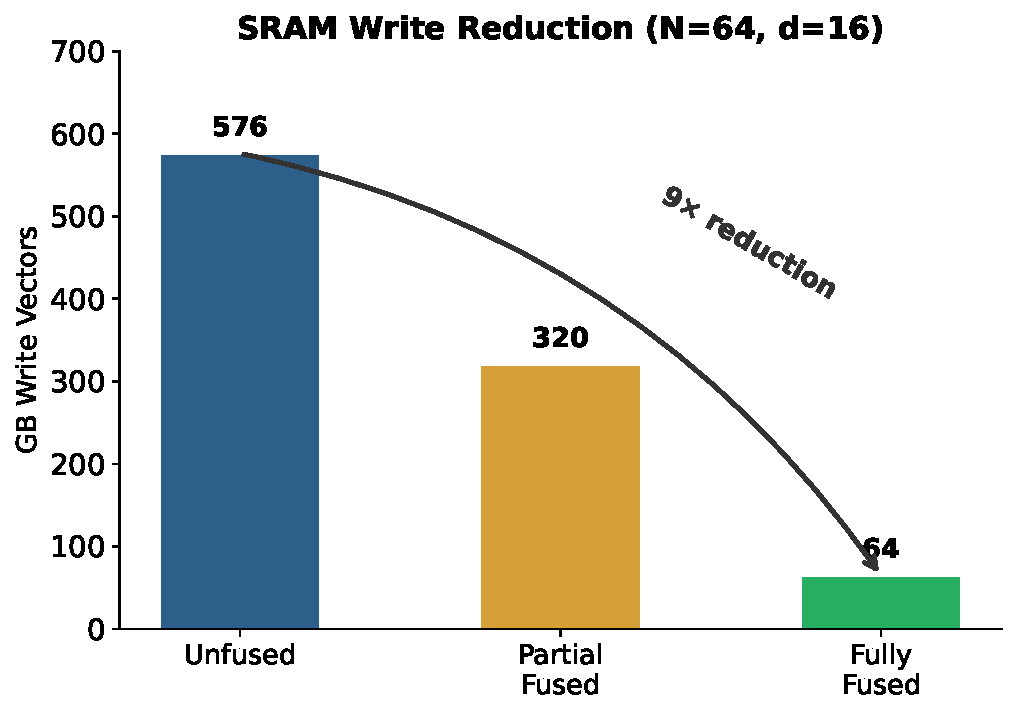
\includegraphics[width=0.75\linewidth]{graph_writes_reduction.pdf}
\caption{GB write vectors for $N=64$, $d=16$. Fully Fused eliminates all intermediate writes, achieving a $9\times$ reduction. The 64 remaining writes are the final $N \times d$ output vectors.}
\label{fig:writes}
\end{figure}

The standard (Unfused) attention flow writes 576 vectors to the GB scratchpad: the $N \times N$ score matrix $S = QK^{T}/\sqrt{d}$ and the $N \times N$ attention weight matrix $A = \mathrm{softmax}(S)$. Partial Fused eliminates the score matrix round-trip ($1.8\times$ reduction), while Fully Fused eliminates \textit{all} intermediate writes ($9\times$ reduction) --- only the final $N \times d$ output is written back.

\subsection*{Latency}

\begin{figure}[h]
\centering
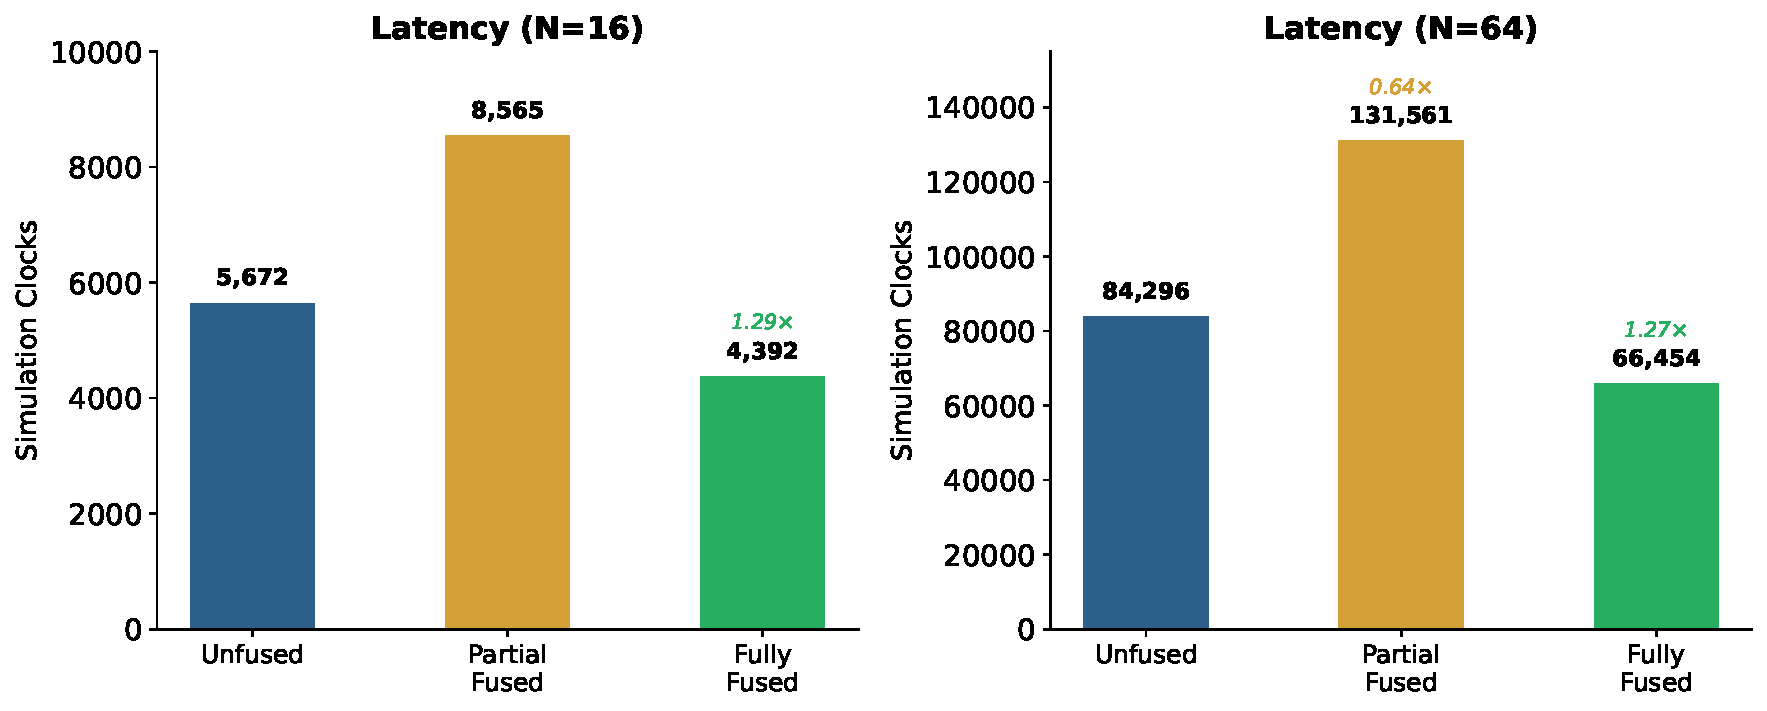
\includegraphics[width=0.95\linewidth]{graph_latency.pdf}
\caption{End-to-end latency (simulation clocks) for $N=16$ and $N=64$. Fully Fused achieves $1.27\times$ speedup; Partial Fused is slowest due to single-port scratchpad contention.}
\label{fig:latency}
\end{figure}

\textbf{Key findings:}
\begin{itemize}
\item \textbf{Fully Fused is $\mathbf{1.27\times}$ faster} than Unfused at $N=64$ (66{,}454 vs.\ 84{,}296 clocks, or 531.6\,$\mu$s vs.\ 674.4\,$\mu$s at 125\,MHz). Despite issuing more GB reads (re-reading $K$ and $V$ per tile), eliminating write stalls more than compensates.

\item \textbf{Partial Fused is the slowest} ($0.64\times$ of Unfused), despite reducing total data movement. Interleaving reads and writes on the single-port GB scratchpad causes ${\sim}2$ stall cycles per access due to port contention. This is the central architectural insight: \textit{fusion strategy must match the memory port topology}. Partial fusion on a single-port scratchpad creates contention that negates the data movement savings.

\item Speedup is consistent across $N=16$ ($1.29\times$) and $N=64$ ($1.27\times$), confirming the benefit is structural rather than size-dependent.
\end{itemize}


\subsection*{Area Cost}

\begin{table}[h]
\centering
\begin{tabular}{lcccc}
\toprule
\textbf{Variant} & \textbf{DSPs} & \textbf{LUTs} & \textbf{HLS Threads} & \textbf{Area Score} \\
\midrule
Unfused        & 96  & 8{,}667  & 1 & 72{,}699 \\
Partial Fused  & 95  & 16{,}650 & 1 & 80{,}015 \\
Fully Fused    & 186 & 17{,}817 & 2 & 141{,}879 \\
\bottomrule
\end{tabular}
\caption{HLS synthesis area estimates (target clock period = 4.0\,ns).}
\label{tab:area}
\end{table}

Fully Fused costs ${\sim}2\times$ the area of Unfused due to duplicated DSP resources for its two concurrent threads. This represents the fundamental trade-off: overlapping memory access with computation requires additional datapath hardware.


\subsection*{FPGA Deployment}

The Fully Fused variant was synthesized and implemented on an \textbf{AWS F2 FPGA} (Xilinx VU47P) using Vivado 2024.1. The design closed timing at 125\,MHz with no negative slack. RTL hardware simulation passed functional verification, confirming the HLS-generated Verilog behaves identically to the SystemC model.


%------------------------------------------------
% CONCLUSION
%------------------------------------------------

\section*{Conclusion}

We demonstrated that kernel fusion significantly reduces data movement for attention on scratchpad-based accelerators, achieving a $9\times$ reduction in SRAM writes and a $1.27\times$ latency improvement with the Fully Fused variant. Critically, we showed that \textit{more fusion is not always better}: Partial Fused performs worse than the Unfused baseline due to port contention on the single-port scratchpad. The right fusion granularity depends on both the algorithmic data reuse pattern and the underlying memory port topology.


%------------------------------------------------
% FUTURE WORK
%------------------------------------------------

\section*{Future Work}

\begin{itemize}

\item \textbf{Larger sequence lengths}: Extending to $N \geq 256$ would exercise the quadratic scaling of unfused attention, amplifying the fusion advantage.

\item \textbf{Multi-head attention}: Support multiple heads to enable full transformer layer acceleration.

\item \textbf{Power estimation}: Quantify energy savings from reduced SRAM access, which dominates power in scratchpad-based architectures.

\item \textbf{Programmable execution}: Replace hardcoded FSMs with an instruction-driven interface to support causal masks and sparse attention patterns.

\end{itemize}


%------------------------------------------------
% REFERENCES
%------------------------------------------------

\section*{References}

\begin{enumerate}

\item T. B. Brown et al., ``Language Models are Few-Shot Learners,'' NeurIPS 2020.

\item A. Vaswani et al., ``Attention Is All You Need,'' NeurIPS 2017.

\item J. Tambe et al., ``EdgeBERT: Sentence-Level Energy Optimizations for Latency-Aware Multi-Task NLP Inference,'' MICRO 2021.

\item T. Dao et al., ``FlashAttention: Fast and Memory-Efficient Exact Attention with IO-Awareness,'' NeurIPS 2022.

\end{enumerate}


\end{document}
